\documentclass[sigplan,screen,10pt]{acmart}
\usepackage[utf8]{inputenc}
\usepackage[T1]{fontenc}
\usepackage[french]{babel}

\begin{document}
	\section*{Number of accesses to cluster}
	
	This describe, the number of accesses to a same cluster per snapshot during a workload.
	I focus here on chain of 50 and 500 snapshots.
	We noticed that in vanilla version, the number of accesses if larger because we are always looking for all the pasts snapshots in order to find a specific cluster.
	
	With our direct-access method, we only have the exact number of accesses which give us the real index and then we can jump to that snapshot index, omitting access to intermediate snapshots.
	
	\begin{figure}[h]
		\center
		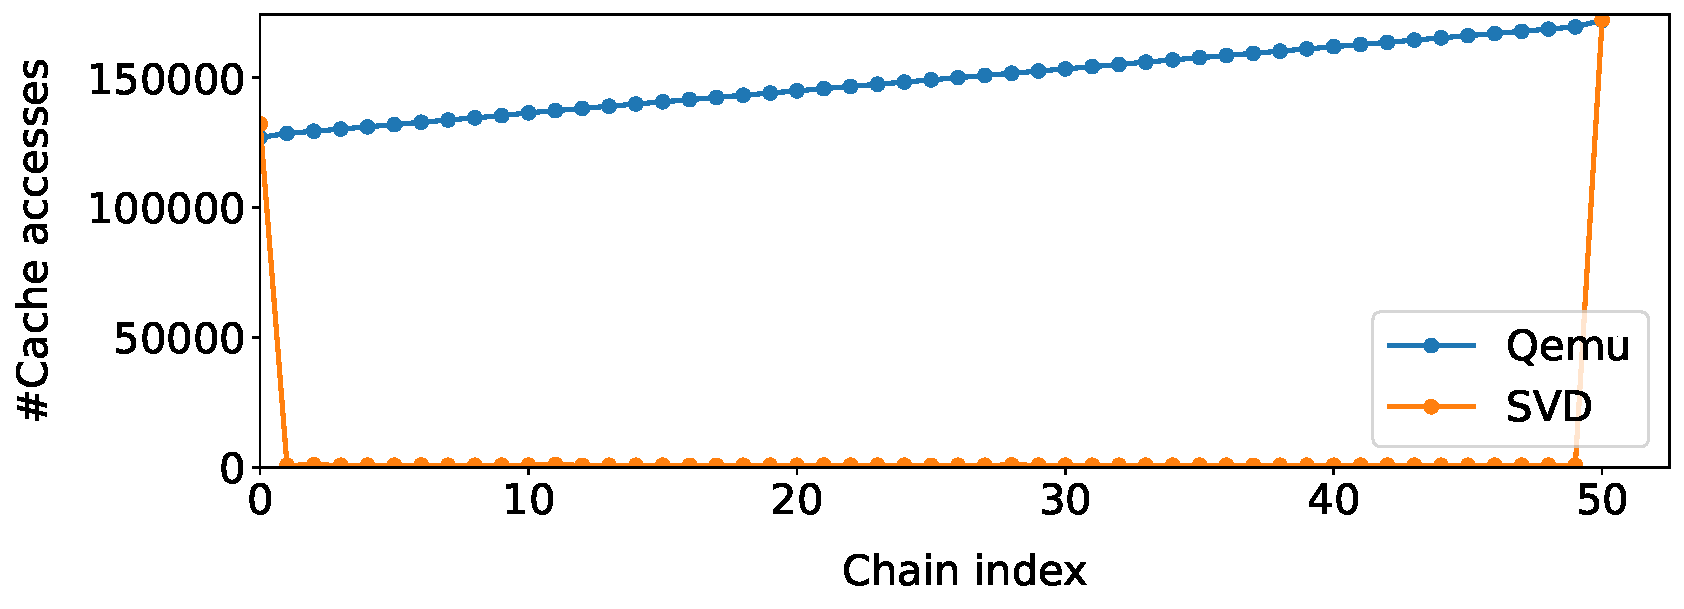
\includegraphics[width=0.45\textwidth]{clusters_accesses_chain_50.pdf}
		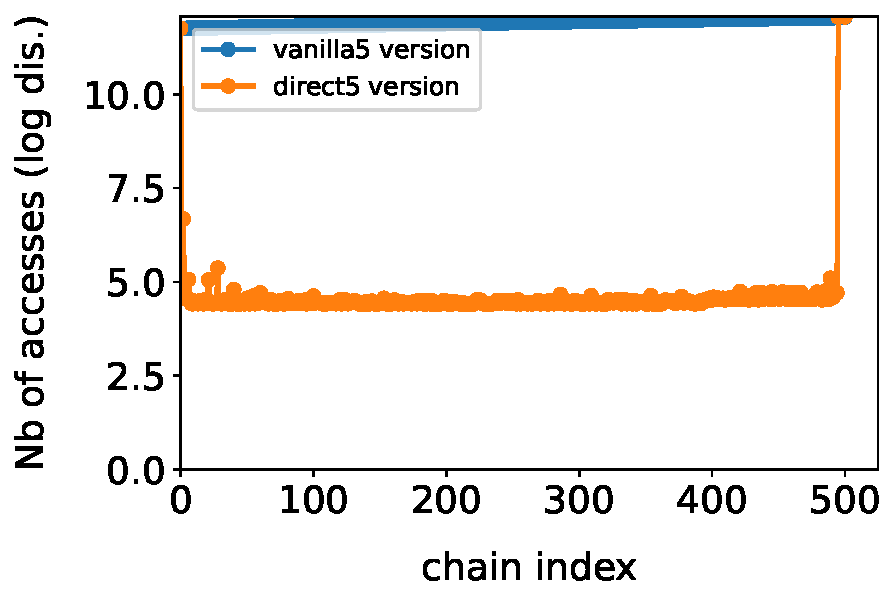
\includegraphics[width=0.45\textwidth]{clusters_accesses_chain_500.pdf}
		\caption{Accesses in a chain of 50 and 500 snap}
		\label{fig:fig2}
	\end{figure}


	\section*{Details on type of accesses to cluster (events)}
	
	Here, we focus on explaining why there are more accesses in vanilla version, and we are doing it by distinguishing all the type of access results (here we call it \textit{event}) in each chain.
	\begin{itemize}
		\item unallocated => the cluster is not allocated in the current snap
		\item normal => the cluster is allocated in the current (occured when we resolve an unallocated event)
		\item hit/missed => relative to the fact that cluster metadata are presented/not presented in the cache
	\end{itemize}
	
	
	\begin{figure}[h]
		\center
		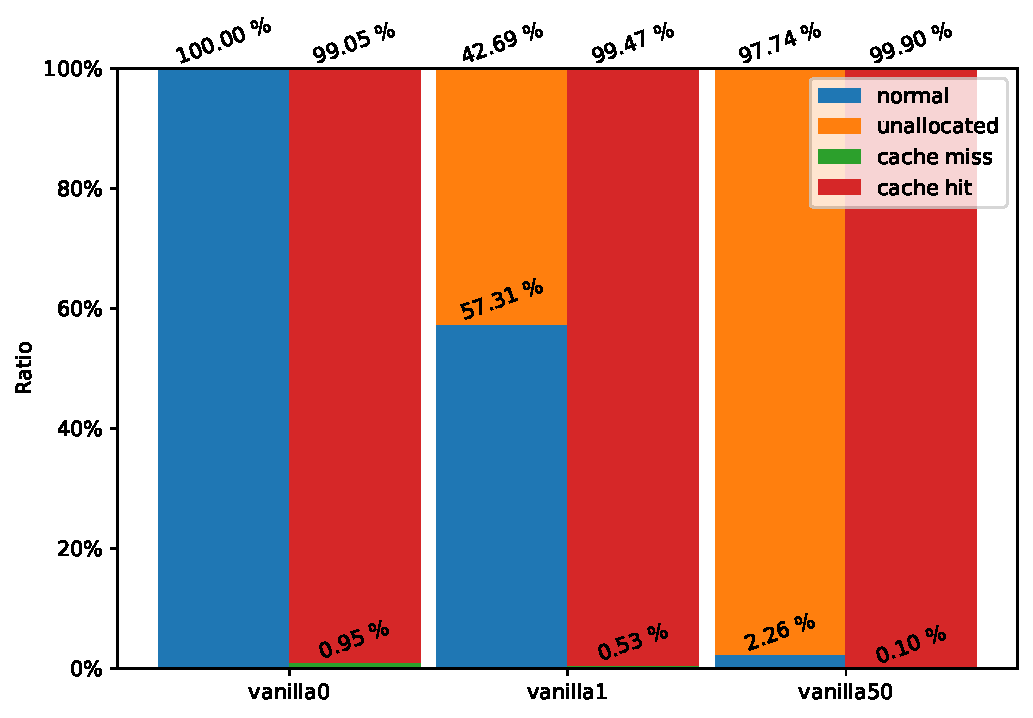
\includegraphics[width=0.6\textwidth]{number_events_per_chain_va.pdf}
		\caption{Number of events (unallocated, missed, hit, normal) for the vanilla version, the number on the x-axis indicate the chain length corresponding}
		\label{fig:fig36}
	\end{figure}

	We noticed that in the vanilla version, the number of unallocated events that we get in order to get the current location of the cluster (normal event occurence) increased exponentially with the chain of the length. While in our direct-access version, we always approximatively have the same number of unallocated and normal event regardless of the chain length, this due to the fact that a same "unallocated event" is not propagate all over the chain like in the vanilla version.
	
	\begin{figure}[h]
		\center
		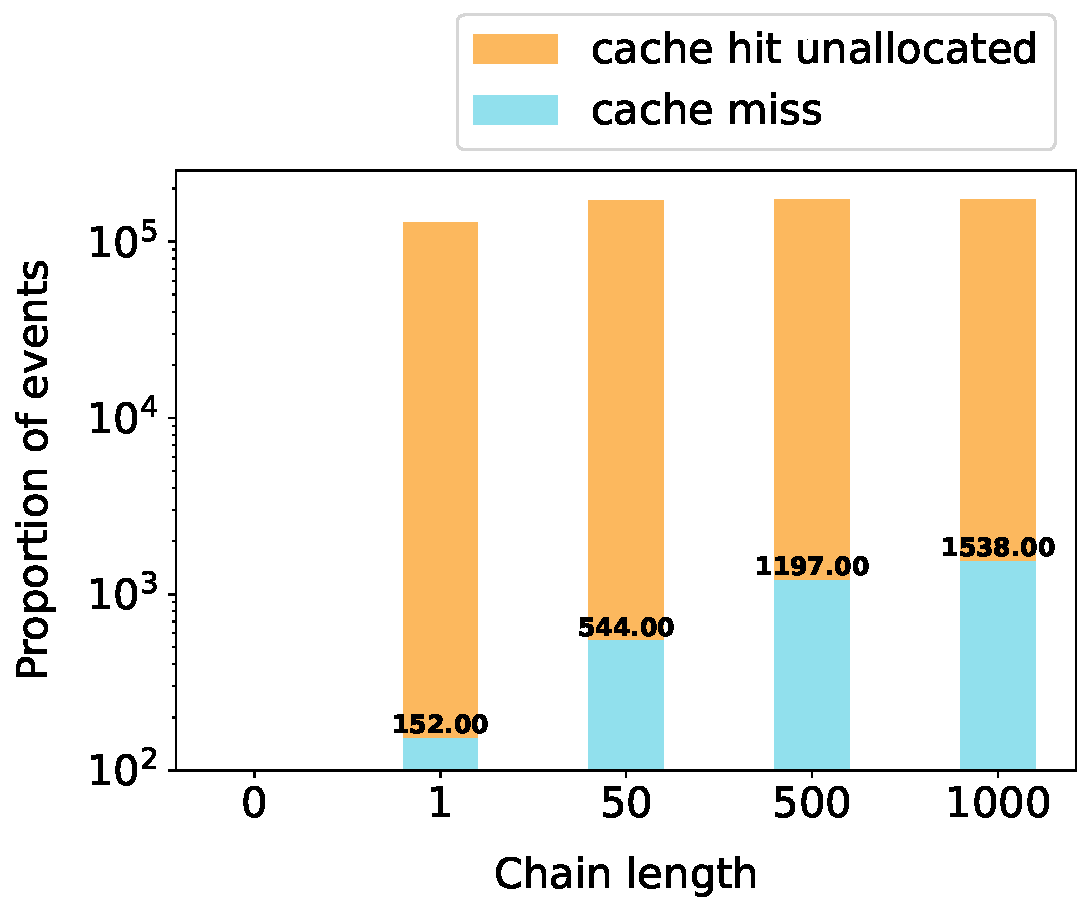
\includegraphics[width=0.6\textwidth]{number_events_per_chain_di.pdf}
		\caption{Number of events (unallocated, missed, hit, normal) in the direct-access version}
		\label{fig:fig36}
	\end{figure}


	\section*{Memory footprint}
	
	Comparison of memory footprint and throughput during workload dd, between our version and the vanilla one.
	
	\begin{figure}[h]
		\center
		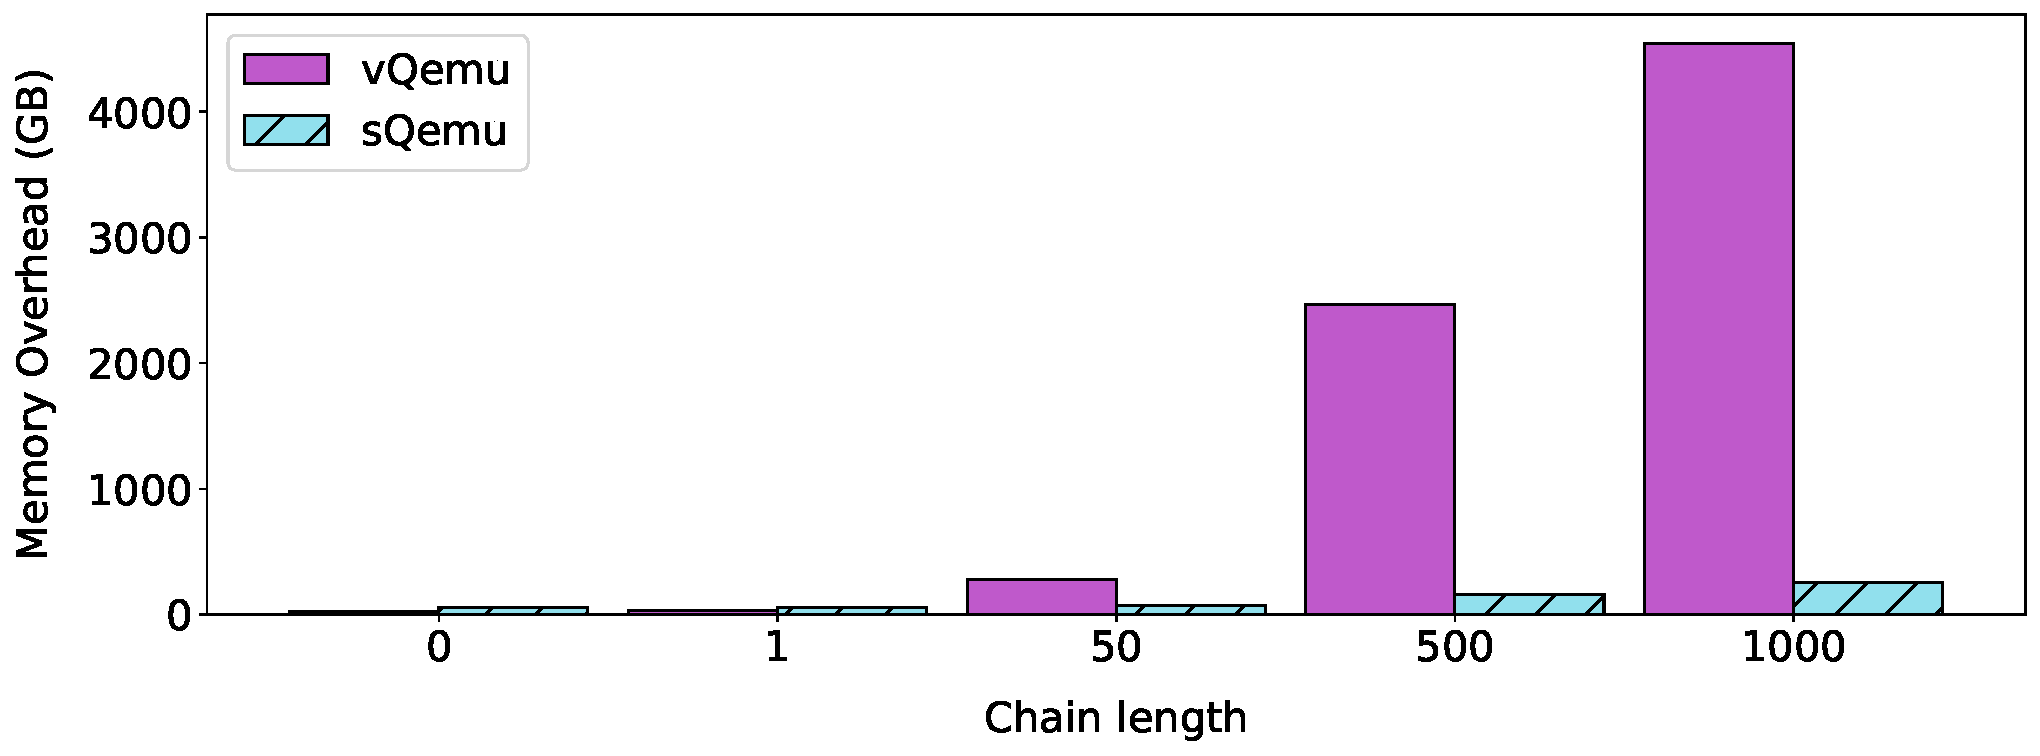
\includegraphics[width=0.45\textwidth]{memory_consumption.pdf}
		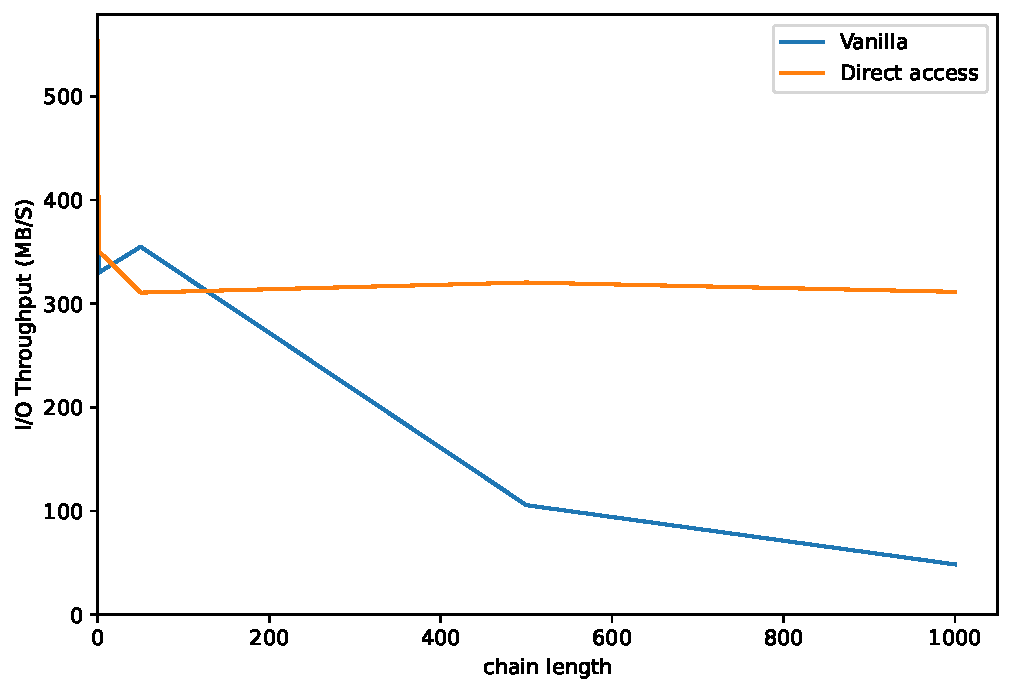
\includegraphics[width=0.45\textwidth]{workload_dd_throughput.pdf}
		\caption{Memory consumption and Throughput (I/O) during all the workload}
		\label{fig:fig3}
	\end{figure}
	
	\section*{Startup duration}
	
	The first evaluation i did:
	
	\begin{figure}[h]
		\center
		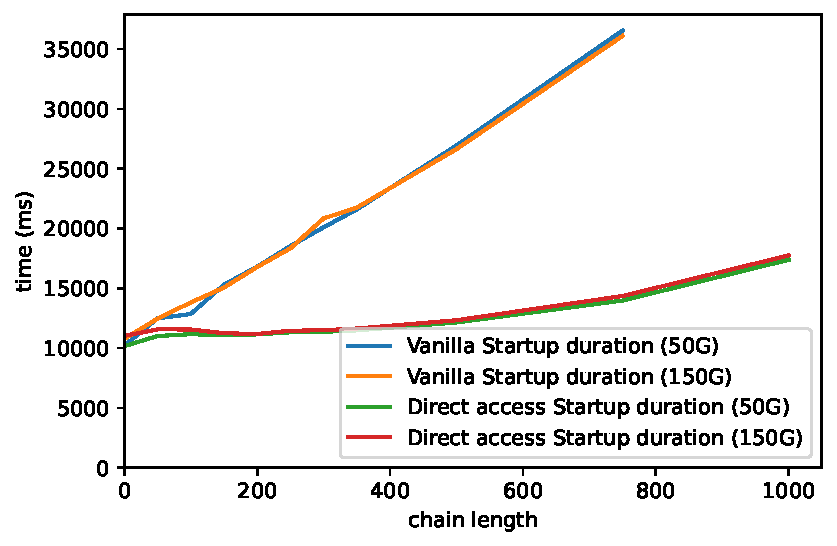
\includegraphics[width=0.45\textwidth]{startup_duration.pdf}
		\caption{Startup, vanilla and direct-access version on 50G and 150G disk}
		\label{fig:fig34}
	\end{figure}

\end{document}